\documentclass[12pt]{article}

\usepackage[utf8]{inputenc}

% Disable paragraph indentation
\usepackage{graphicx}

% For hyperlinks in figure captions
\usepackage{hyperref}

% Disable paragraph indentation
\setlength{\parindent}{0pt}

% Set the length of space between paragraphs
\setlength{\parskip}{12pt}

% Disable page numbering
\pagenumbering{gobble}

% For forcing figure position
\usepackage{float}


\title{Internet of Things - Homework - Question 11}
\author{Francesco Pastore 10629332}
\date{05-14-2024}

\begin{document}

\maketitle

\textbf{Question}

You have setup a weather monitoring station on your balcony and would like to transmit the acquired data over a web service (e.g., ThingSpeak).
You have no Wi-Fi connectivity at home, therefore you plan to use a long-range IoT communication technology.
After careful consideration, you need to choose between LoRa and NB-IoT

11. You opt to use LoRa, using an open-source gateway close by (e.g., provided by the Things Network).
However, your transmission are not successfull. What are the possible causes, and what kind of solutions could be adopted?

\textbf{Answer}

Firstly, the gateway may be too far away, or there may be a physical interference that weakens the signal.
A possible solution could be to move the device to another location with a better line of sight to the gateway.

Another reason could be that the spreading factor currently used is too low (Figure 1).
Using a higher spreading factor may give better reliability, but at a lower transmission rate.

There may also be too many other devices using the same frequency band, causing interference.
In this case, another band could be used in the hope that it is less crowded.

Addiitonaly, the selected gateway may be overloaded and unable to handle the traffic.
In this case, another gateway could be selected based on traffic load.

Another possible cause could be the type of class used by the device.
A class A device generally has the lowest latency but is less reliable.
On the other hand, a class C device is more reliable but has a higher latency.

\begin{figure}[h]
    \centering
    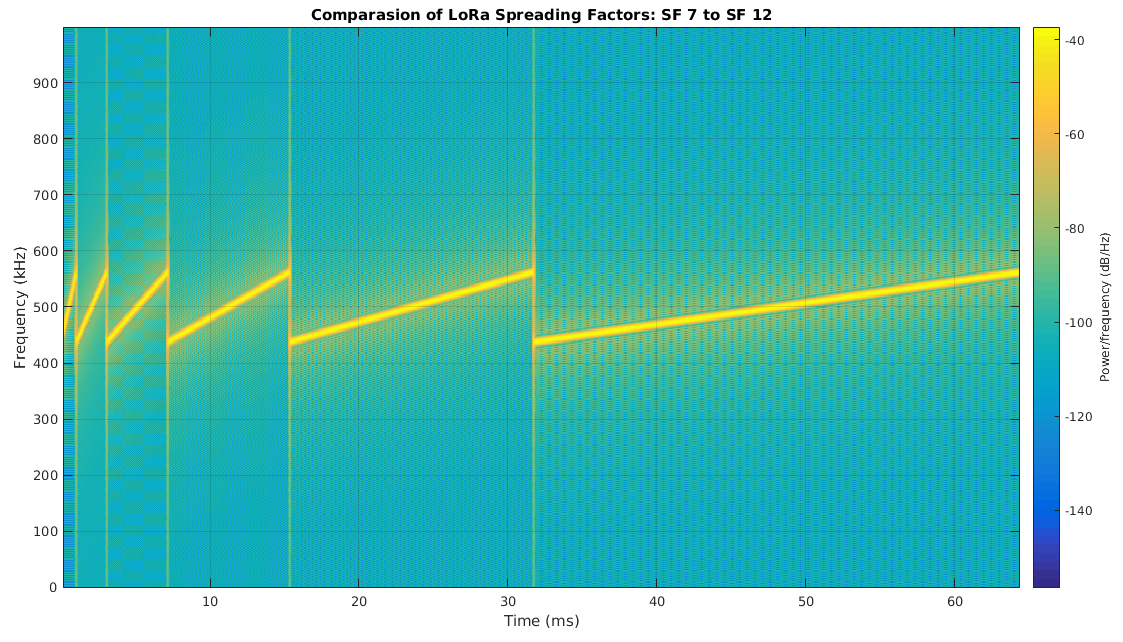
\includegraphics[width=0.8\textwidth]{./spreading-factor.png}
    \caption{Comparison of LoRa spreading factors}
\end{figure}

\end{document}
